\begin{figure}[!htbp]
\centering
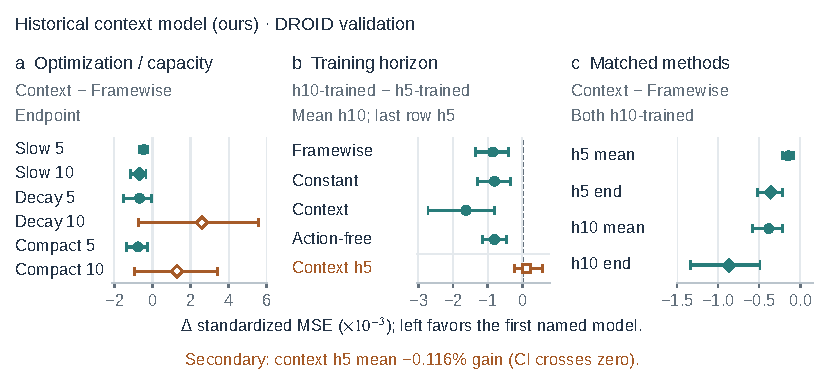
\includegraphics[width=\linewidth]{generated/editorial/validation_controls_compact.pdf}
\caption{\textbf{Optimization, capacity and horizon controls for the historical context model (ours), on original DROID validation.}
Context denotes the factorized two-context model; Constant denotes Constant dynamics.
(a) Context minus matched Framewise endpoint MSE under Slow, Decay and Compact interventions, at five or ten action blocks. All 36 runs train 30 epochs and use the common five-query selection objective; Compact changes predictor and context capacity jointly.
(b) Ten-query-trained minus original five-query-trained mean MSE on identical ten-query-eligible windows, for every method. The separated final row retains the unfavorable matched-five-query Context secondary result ($-0.116\%$ relative gain). Training and selection horizons change together.
(c) Context minus equally ten-query-trained Framewise on standard populations. Mean averages query errors; end denotes the endpoint. All 12 horizon-study runs train 30 epochs; every selected checkpoint is epoch 1.
Bars are paired 95\% session/seed bootstrap intervals (10,000 draws); open marks include zero. Axes use different limits but the same MSE unit. Windows are averaged within 141 episodes from 59 sessions and then three seeds equally. Standard h5 uses 1,772 windows; h10 and matched h5 prefixes use 1,631.
All four-method absolute errors remain in Tables~\ref{tab:generalization-development}, \ref{tab:h10-native-endpoint} and~\ref{tab:h10-native-mean}; all 20 registered horizon contrasts remain in the tables and companion ledger. These exploratory, multiplicity-unadjusted comparisons provide no independent-test claim.}
\label{fig:generalization-summary}
\label{fig:horizon10_summary}
\end{figure}
